\documentclass[psamsfonts]{amsart}

%-------Packages---------
\usepackage{amssymb,amsfonts}
\usepackage[all,arc]{xy}
\usepackage{enumerate}
\usepackage{mathrsfs}
\usepackage[margin=1in]{geometry}
\usepackage{thmtools}
\usepackage{verbatim}
\usepackage{multirow}
\usepackage{tikz}
\usetikzlibrary{shapes,arrows}


%--------Theorem Environments--------
%theoremstyle{plain} --- default
\newtheorem{prob}{Problem}[section]
\newtheorem{thm}{Theorem}[section]
\newtheorem{cor}[thm]{Corollary}
\newtheorem{prop}[thm]{Proposition}
\newtheorem{lem}[thm]{Lemma}
\newtheorem{conj}[thm]{Conjecture}
\newtheorem{quest}[thm]{Question}

\newenvironment{sol}{{\bfseries Solution}}{\qedsymbol}


\theoremstyle{definition}
\newtheorem{defn}[thm]{Definition}
\newtheorem{defns}[thm]{Definitions}
\newtheorem{con}[thm]{Construction}
\newtheorem{exmp}[thm]{Example}
\newtheorem{exmps}[thm]{Examples}
\newtheorem{notn}[thm]{Notation}
\newtheorem{notns}[thm]{Notations}
\newtheorem{addm}[thm]{Addendum}
\newtheorem{exer}[thm]{Exercise}

\theoremstyle{remark}
\newtheorem{rem}[thm]{Remark}
\newtheorem{rems}[thm]{Remarks}
\newtheorem{warn}[thm]{Warning}
\newtheorem{sch}[thm]{Scholium}

\makeatletter
\let\c@equation\c@thm
\makeatother
\numberwithin{equation}{section}

\bibliographystyle{plain}

\voffset = -10pt
\headheight = 0pt
\topmargin = -20pt
\textheight = 690pt

%--------Meta Data: Fill in your info------
\title{6.046 \\
Problem Set 2}

\author{John Wang}

\begin{document}

\maketitle

Collaborators: Sashko Stubailo

\section{Problem 1}
Let $G = (V,E)$ be a connected, weighted undirected graph whose edges weight may or may not
be distinct. Given a cut $(S, V - S)$ of $S$, recall that an edge $(u, v) \in E$ is said to cross the cut
if exactly one of $u$ and $v$ is in $S$. An edge $(u, v)$ is a light edge crossing the cut $(S, V - S)$ if its
weight is the smallest of any edge crossing $(S, V - S)$. There can be more than one light edge
crossing a single cut in the case of ties. An edge $(u, v)$ is a unique light edge if there are no ties.

\begin{prob}
Show that if an edge $(u, v)$ is the unique light edge crossing some cut of the connected,
weighted undirected graph $G$, then $(u, v)$ must be included in all minimum spanning
trees of $G$.
\end{prob}

\begin{sol}
Suppose by contradiction that there exists some minimum spanning tree $M$ which does not include $(u,v)$. Then in order to corss the cut $(S, V - S)$, $M$ must include some other edge $(x,y)$ which has weight greater than $(u,v)$ where either $x \neq u$ or $v \neq y$. Let $p$ be the path connecting vertices $u$ and $v$ in $M$. This path must contain $(x,y)$ because the path must cross $(S, V - S)$, and it cannot pass through $(u,v)$. If we remove the edge $(x,y)$ and add the edge $(u,v)$ to the path to create $M^*$. Note that all vertices $u \in V$ will still be connected in the tree $M^*$. This is because the set $M \setminus (x,y)$ consists of two connected subsets $S$ and $V - S$, and adding the $(u,v)$ edge will reconnect these subsets.

However, we know that $w((x,y)) > w((u,v))$. This means that $M^*$ now has a weight $w(M^*)$ such that 
\begin{eqnarray}
w(M^*) &=& w((u,v)) + \sum_{(w,z) \in M^{*}} w((w,z)) \\
&<& w(M) = w((x,y)) + \sum_{(w,z) \in M} w((w,z))
\end{eqnarray}

This is a contradiction because $M^*$ has a lower weight than $M$, which is a minimum spanning tree. Thus, there does not exist a minimum spanning tree $M$ which does not include $(u,v)$. 
\end{sol}

\begin{prob}
Suppose that we have a connected, weighted undirected graph $G = (V,E)$ such that
every cut of $G$ has a unique light edge crossing the cut. Show that $G$ has exactly one
minimum spanning tree.
\end{prob}

\begin{sol}
First, it is clear by the definition of a minimum spanning tree that at least one exists for a connected, weighted, undirected graph. Now, assume by contradiction that there exist $n > 1$ minimum spanning trees. Then we can construct a minimum spanning tree in the following manner.

Start with some arbitrary vertex $u_0$. Let $S_0 = \{ u_0 \}$. By assumption, there exists a vertex $u_1$ such that $(u_0, u_1)$ is the unique light edge crossing the cut $(S_0, V - S_0)$. Thus, $(u_0, u_1)$ is a unique light edge and by the previous theroem, it must be included in all $n$ minimum spanning trees. 

Next, we use the set $S_1 = \{ u_0, u_1 \}$. There exists a $u_2$ such that $(u_i, u_2)$ is the unique light edge crossing the cut $(S_1, V - S_1)$ for some $i \in \{0, 1 \}$. The edge $(u_i, u_2)$ must belong to every minimum spanning tree by the theorem proven above. What is more, the tree $T^* = \{ (u_0, u_1), (u_i, u_2) \}$ must be a subset of every minimum spanning tree. 

We can continue to perform this operation until all vertices $u \in V$ are inside of the tree $T^*$, which is a susbet of every minimum spanning tree. However, we see that $T^*$ is a connected, undirected tree which contains each vertex $u \in V$ exactly once. There are no cycles because we have defined each new edge in $T^*$ to cross cuts $(S_i, V - S_i)$ where $S_i$ contained all previously connected vertices. Hence, $T^*$ is itself a minimum spanning tree. 

However, we see that no minimum spanning tree can have any more edges than $T^*$ (since another edge would create a cycle) or vertices than $T^*$ (since it already contains all vertices in $V$). Thus, we see that $T^*$ is exactly equal to each one of the $n$ minimum spanning trees since $T^*$ is both a subset of $M_i$ (the $i$th minimum spanning tree), and $M_i$ is a subset of $T^*$. This implies that there exists only a single unique minimum spanning tree, which is a contradiction.
\end{sol}

\section{Problem 2}

In this problem, you will examine the relationship between minimum spanning trees and shortest
path trees. As a reminder, given a weighted undirected graph $G = (V,E)$ with edge weights $w$,
the shortest path tree rooted at $s \in V$ is a subgraph $G' = (V',E')$ of $G$ such that:
\begin{enumerate}
\item The vertex set $V' \subset V$ is the set of nodes in $G$ reachable from $s$.
\item The graph $G'$ is a tree, with $|E'| = |V'| - 1$.
\item For any $u \in V'$, the distance from $s$ to $u \in G'$ is the same as the distance from $s$ to $u$ in $G$.
\end{enumerate}
Note that as with minimum spanning trees, there is more than one shortest path tree per graph. In
addition to the variation introduced by the choice of root, it's possible to get different shortest path
trees even for the same root vertex.

\begin{prob}
Given any connected undirected graph $G$ with positive edge weights $w$, does there
always exist a shortest path tree $S$ such that $S$ is a minimum spanning tree of $G$?
Prove your answer.
\end{prob}

\begin{sol}
There does not always exist a shortest path tree $S$ such that $S$ is a minimum spanning tree as well. We will show this using the following counter-example. 

\tikzstyle{line} = [draw, -, >=latex, line width=0.5pt]
\tikzstyle{boldline} = [draw, -, >=latex, line width=4pt]
\tikzstyle{cloud} = [draw, circle, distance=3cm, minimum height=2em]

\begin{figure}[h!]
\centering
\begin{tabular}{c c  c}
\begin{tikzpicture}[node distance=2cm, auto]
    \node [cloud] (n1) {Node 1};
    \node [cloud, left of=n1] (n2) {Node 2};
    \node [cloud, right of=n1] (n3) {Node 3};
    \node [cloud, below of=n2] (n4) {Node 4};
    \node [cloud, below of=n3] (n5) {Node 5};
    % Draw edges
    \path [line] (n1) -- node [below=2] {2} (n2);
    \path [line] (n1) -- node [below=2] {2} (n3);
    \path [line] (n2) -- node {2} (n4);
    \path [line] (n3) -- node [left=2] {2} (n5);
    \path [line] (n1) -- node [below=5] {3} (n4);
    \path [line] (n1) -- node [below=5] {3} (n5);
\end{tikzpicture}
&  \hspace{0.5cm} &
\begin{tikzpicture}[node distance=2cm, auto]
    \node [cloud] (n1) {Node 1};
    \node [cloud, left of=n1] (n2) {Node 2};
    \node [cloud, right of=n1] (n3) {Node 3};
    \node [cloud, below of=n2] (n4) {Node 4};
    \node [cloud, below of=n3] (n5) {Node 5};
    % Draw edges
    \path [boldline] (n1) -- node [below=2] {2} (n2);
    \path [boldline] (n1) -- node [below=2] {2} (n3);
    \path [boldline] (n2) -- node {2} (n4);
    \path [boldline] (n3) -- node [left=2] {2} (n5);
    \path [line] (n1) -- node [below=5] {3} (n4);
    \path [line] (n1) -- node [below=5] {3} (n5);
\end{tikzpicture}\\
Counter-Example Graph & \hspace{0.5cm} & Minimum Spanning Tree 
\end{tabular}
\end{figure}

It can be seen by inspection that the above graph has a single, unique minimum spanning three. This is given above on the right side. The minimum spanning tree is demarcated by bold lines. Now, we will show all the possible shortest path trees. Note that for each node, there exists a unique shortest path tree, which will make it easier to display all of them. Below, we display each of the shortest path trees rooted at all 5 of the possible nodes. The bolded lines correspond to the shortest paths tree. Also note that SPT is short for shortest path tree.

\begin{figure}[h!]
\centering
\begin{tabular}{c c c}
\begin{tikzpicture}[node distance=2cm, auto]
    \node [cloud] (n1) {Node 1};
    \node [cloud, left of=n1] (n2) {Node 2};
    \node [cloud, right of=n1] (n3) {Node 3};
    \node [cloud, below of=n2] (n4) {Node 4};
    \node [cloud, below of=n3] (n5) {Node 5};
    % Draw edges
    \path [boldline] (n1) -- node [below=2] {2} (n2);
    \path [boldline] (n1) -- node [below=2] {2} (n3);
    \path [line] (n2) -- node {2} (n4);
    \path [line] (n3) -- node [left=2] {2} (n5);
    \path [boldline] (n1) -- node [below=5] {3} (n4);
    \path [boldline] (n1) -- node [below=5] {3} (n5);
\end{tikzpicture}
& \hspace{0.5cm} &
\begin{tikzpicture}[node distance=2cm, auto]
    \node [cloud] (n1) {Node 1};
    \node [cloud, left of=n1] (n2) {Node 2};
    \node [cloud, right of=n1] (n3) {Node 3};
    \node [cloud, below of=n2] (n4) {Node 4};
    \node [cloud, below of=n3] (n5) {Node 5};
    % Draw edges
    \path [boldline] (n1) -- node [below=2] {2} (n2);
    \path [boldline] (n1) -- node [below=2] {2} (n3);
    \path [boldline] (n2) -- node {2} (n4);
    \path [line] (n3) -- node [left=2] {2} (n5);
    \path [line] (n1) -- node [below=5] {3} (n4);
    \path [boldline] (n1) -- node [below=5] {3} (n5);
\end{tikzpicture} \\

SPT Rooted at Node 1 & \hspace{0.5cm} & SPT Rooted at Node 2 \\

\begin{tikzpicture}[node distance=2cm, auto]
    \node [cloud] (n1) {Node 1};
    \node [cloud, left of=n1] (n2) {Node 2};
    \node [cloud, right of=n1] (n3) {Node 3};
    \node [cloud, below of=n2] (n4) {Node 4};
    \node [cloud, below of=n3] (n5) {Node 5};
    % Draw edges
    \path [boldline] (n1) -- node [below=2] {2} (n2);
    \path [boldline] (n1) -- node [below=2] {2} (n3);
    \path [line] (n2) -- node {2} (n4);
    \path [boldline] (n3) -- node [left=2] {2} (n5);
    \path [boldline] (n1) -- node [below=5] {3} (n4);
    \path [line] (n1) -- node [below=5] {3} (n5);
\end{tikzpicture}
& \hspace{0.5cm} &
\begin{tikzpicture}[node distance=2cm, auto]
    \node [cloud] (n1) {Node 1};
    \node [cloud, left of=n1] (n2) {Node 2};
    \node [cloud, right of=n1] (n3) {Node 3};
    \node [cloud, below of=n2] (n4) {Node 4};
    \node [cloud, below of=n3] (n5) {Node 5};
    % Draw edges
    \path [line] (n1) -- node [below=2] {2} (n2);
    \path [boldline] (n1) -- node [below=2] {2} (n3);
    \path [boldline] (n2) -- node {2} (n4);
    \path [line] (n3) -- node [left=2] {2} (n5);
    \path [boldline] (n1) -- node [below=5] {3} (n4);
    \path [boldline] (n1) -- node [below=5] {3} (n5);
\end{tikzpicture} \\

SPT Rooted at Node 3 & \hspace{0.5cm} & SPT Rooted at Node 4
\end{tabular}
\end{figure}

\begin{figure}[h!]
\centering
\begin{tabular}{c}
\begin{tikzpicture}[node distance=2cm, auto]
    \node [cloud] (n1) {Node 1};
    \node [cloud, left of=n1] (n2) {Node 2};
    \node [cloud, right of=n1] (n3) {Node 3};
    \node [cloud, below of=n2] (n4) {Node 4};
    \node [cloud, below of=n3] (n5) {Node 5};
    % Draw edges
    \path [boldline] (n1) -- node [below=2] {2} (n2);
    \path [line] (n1) -- node [below=2] {2} (n3);
    \path [line] (n2) -- node {2} (n4);
    \path [boldline] (n3) -- node [left=2] {2} (n5);
    \path [boldline] (n1) -- node [below=5] {3} (n4);
    \path [boldline] (n1) -- node [below=5] {3} (n5);
\end{tikzpicture} \\
SPT Rooted at Node 5
\end{tabular}
\end{figure}

From the above figures, it is clear that none of the shortest path trees correspond to the minimum spanning tree shown in the first diagram. This means that for any connected, undirected graph $G$ with positive edge weights, there does not necessarily exist a shortest path tree $S$ such that $S$ is a minimum spanning tree of $G$. 
\end{sol}

\begin{prob}
Does there exist some connected undirected graph $G$ with positive edge weights $w$
such that $G$ has a shortest path tree $S$ and a minimum spanning tree $T$ that do not
share any edges? Prove your answer.
\end{prob}

\begin{sol}
Yes, there does exist a shortest path tree $S$ and a minimum spanning tree $T$ that do not share any edges. Consider the following simple example:
\begin{figure}[h!]
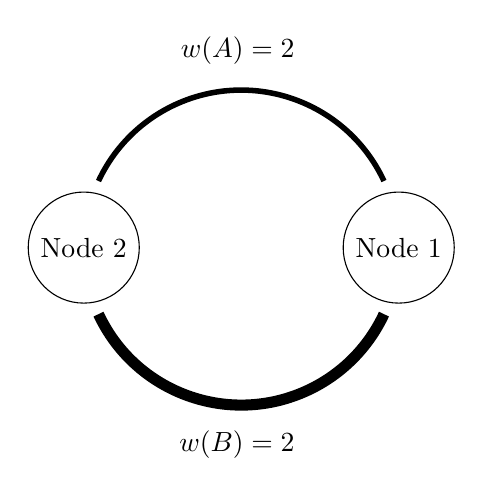
\begin{tikzpicture}
\def \n {2}
\def \radius {2cm}
\def \margin {25}

\foreach \s in {1,...,\n}
{
  \node[draw, circle] at ({360/\n * (\s - 1)}:\radius) {Node $\s$};
  \draw[-, line width=(2* \s), >=latex] ({360/\n * (\s - 1)+\margin}:\radius) 
    arc ({360/\n * (\s - 1)+\margin}:{360/\n * (\s)-\margin}:\radius); 
}

\draw[dashed] (0.8,2.5) node[left] {$w(A) = 2$};
\draw[dashed] (0.8,-2.5) node[left] {$w(B) = 2$};
\end{tikzpicture}
\caption{Shortest Path and Minimum Spanning Trees}
\end{figure}

Here, we see that there is a shortest path tree $S$ consisting of the edge $A$. This tree is on the top of the image and contains a thin line of weight 2. A minimum spanning tree $S$ consists of the edge $B$ and is at the bottom of the image with a thicker line of weight 2. Clearly, the shortest path from node 1 to 2 must have weight 2. Moreover, the minimum spanning tree of this graph must also have weight 2. Thus, it is clear that $S$ is an acceptable shortest path tree with weight 2 and connecting nodes 1 and 2. It is also clear that $T$ is an acceptable minimum spanning tree with weight 2 and connecting nodes 1 and 2. However, we see that $S$ and $T$ do not share any edges. 
\end{sol}

\end{document}